\documentclass[10 pt]{scrartcl}

%%%%%%%%%%%%%%%%%%%%%%%%%%
% commonly used packages %
%%%%%%%%%%%%%%%%%%%%%%%%%%

% for setting the margins
\usepackage[margin=1 in]{geometry}
% for typing equations and mathematical symbols
\usepackage{amssymb, mathtools}
% for using tikz to plot graphs and draw figures
\usepackage{tikz, pgfplots}
% for creating elegant tables and figures
\usepackage{booktabs, float, multirow, caption, array}
% for including citations
\usepackage{cite}
% for highlighting text
\usepackage{soul}
% for typing physics and mathematical symbols
\usepackage[boldvectors]{physymb}
% for customizing the enumerate environment
\usepackage{enumerate}
% for using bold in special cases
\usepackage{bm}

%%%%%%%%%%%%%%%%%%%%%%%%%%
% commonly used settings %
%%%%%%%%%%%%%%%%%%%%%%%%%%

% sets pgfplots to use the newest version
\pgfplotsset{compat=newest}

%sets KOMA to use the same standard font as the 'article' document class
\addtokomafont{disposition}{\rmfamily}

\title{Flipbook Animator}
\subtitle{CS 242: Advanced Programming Concepts in Java}
\author{Will Havelin \and Michael Tillotson \and Andr\'{e}s Rivas \and Dalton Patterson}
\date{December 7, 2014}

% miscellaneous math shortcuts
\newcommand{\p}[1]{\left(#1\right)}
\newcommand{\br}[1]{\left[#1\right]}

\begin{document}

\maketitle

\section{Introduction}

The purpose of this project was to develop a desktop application that allows the user to create and view digital flipbooks. These flipbooks consist of a series of images that are shown one after the other at a fast rate in order to give the appearance of motion. We developed a program called FlipBook Animator that runs on Windows, Linux and Mac OS.

\section{Problem Description}

The functional requirements for the program are as follows:
\begin{enumerate}
    \item The user must be able to draw images.
    \item The system must save those images as frames that make up a flipbook.
    \item The user must be able to view flipbooks.
    \item The user must be able to export and save their flipbooks.
\end{enumerate}
In addition to these functional requirements, we also wanted our system to be very easy to use and have a nice cohesive feel. A more detailed description of the project can be found in the user manual included with this project.

\section{Methodology}

We broke the system up into different subsystems, which were assigned to different group members. We tried to minimize coupling between subsystems, so as to make our system design as clean as possible. We considered using the Observer design pattern, but decided against using it because we felt that the benefits would not justify the significant increase in development time that using it would require. Initially, we had the drawing and GUI subsystems as separate classes, but later merged them together because the drawing functionality is the main part of the program, while the playback can be handled by a backend class that just tells the GUI what image to display at what time.

\section{Implementation}

\begin{itemize}
    \item The tasks were divided into four separate sections: GUI, Drawing, Playback, and File Management. The sections were worked on by Dalton Patterson, Michael Tillotson, Will Havelin, and Andr\'{e}s Rivas, respectively.
    \item For this project, Dalton, Michael, and Will used Eclipse 4.4 as an IDE, while Andr\'{e}s used NetBeans 8.0. Dalton used the open source image editor GIMP to draw the button icons. Will used the open source diagram editor Dia to draw our UML diagram and we used GitHub as our version control system.
    \item Five source code files are used in the FlipBook program:
    \begin{enumerate}
        \item Flipbook.java creates the GUI and runs all the drawing functions.
        \item Playback.java tells FlipBook.java what images to show at what time during playback.
        \item SaveAndRender.java handles saving the user's work to a zip file and rendering to GIF files. 
        \item GifSequenceWriter.java handles the rendering details.
        \item Dialog.java contains a skeleton for displaying basic message dialogs to the user.
    \end{enumerate}
    Also, flipbookStyle.css skins the GUI created in FlipBook.java.  The icons used by the program are a set of PNG files.
    \item We did integration testing of the combined system on Windows, Mac OS, and Linux. We tested all functionality of our system on all expected use cases.
    \item We have included a UML diagram detailing our subsystems below:
    \begin{figure}[H]
        \centering
        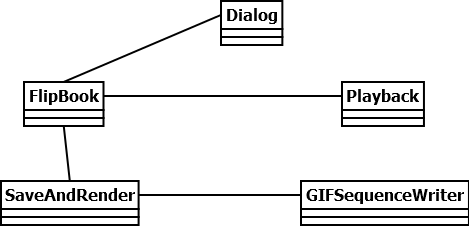
\includegraphics[width=0.75\textwidth]{flipbookUML}
        \caption{A UML diagram of the Flipbook Animator program.}
    \end{figure}
\end{itemize}

\section{Discussion}

\subsection{GUI -- Dalton Patterson}

For my portion of the project I designed a simple GUI based on the implemented functions of the program and my own knowledge of similar systems in other programs.  I used simple css styling to edit the program's buttons to react to being moused over and clicked, providing the user with clear feedback from the program.  A problem with the initial, unstyled program was that a blank space existed to the right of the buttons, indistinguishable from the usable canvas.  To fix this, I styled the root with the same background color as the buttons, creating a toolbar which looks smooth and is clearly differentiated from the canvas.  This required a slight reorganization of the scene declaration but nothing intensive.

I also spent a bit of time studying common image processing iconography to help inspire what the icons for our program's buttons should look like.  I decided to make the icons for the program myself for a number of reasons.  Firstly, it ensures a high-quality, cohesive style for the entire toolbar that may be adjusted as needed.  Secondly, it eliminates concerns regarding the use of third-party content in our program.  Thirdly, it was actually easier in my opinion to make my own icons rather than search for an icon set online that met my aesthetic and formatting standards.

\subsection{Drawing -- Michael Tillotson}

The biggest challenge when implementing the drawing features was being able to see previews when drawing a line. Currently the program draws a dot at the point when the mouse first clicks and draws a line from the dot to the point where the mouse releases. Before I had a preview of the line that would erase and redraw itself every time the mouse moved. This worked for the preview but caused issues when going over another area of the drawing. When the line passed over another section of the drawing it would also erase that part alone with the line.

Another challenge was getting the circles to work. In JavaFX, the \verb|strokeOval| command takes the starting x and y point along with a width and length. Then it strokes the circle from the point which happens to be in the upper left corner. This led to some problems with the circle not drawing where you would expect it to be. Extremely so if you clicked and went up and to the left making the initial click the bottom right point.

\subsection{Playback - Will Havelin}

For me most of the challenges with this project were on the group communication and project management side as opposed to the technical. I found coordinating between different group members to be frustrating at times. In the end, much of the planned functionality was not able to be included in the final product, largely because of group coordination issues.  The biggest feature we had to scrap was the timeline subsystem which would allow the user to select which frame they are working on. This would have been a great feature for a system to have, but it was not essential.

From a technical side, the main challenge was to designing my subsystem and helping design the entire
system. Fairly late in the development process, I did some restructuring of subsystem in order to make
it easier to integrate into the full system. It was not ideal to have to restructure my code, but I felt that
it was justified because it made my subsystem have an interface that was much easier to work with.

\subsection{File Management -- Andr\'{e}s Rivas}

The File Management subsystem is responsible for tasks related to file input and output. This includes saving the user's progress to a zip file, loading a previously saved zip file so the user can continue working on his or her flipbook, and rendering the user's work to an animated GIF file.

For saving and loading the user's work, the zip file was chosen for simplicity, since the Java standard library already has functionality for reading from and writing to zip files. Since the frames are stored internally as a List of Image objects, the frames are simply written to zip entries named ``Page\_$i$.png," where $i$ is the index of the frame, and the entries are written to the zip file. Originally, the program was going to offer support for a background image that would be overlayed with the frames at the time of rendering. Therefore, the saving functionality was implemented so that, if a background image is supplied, then it is also saved to the zip file with the name ``background.png."

The biggest challenge was finding and using suitable third-party code for rendering the GIF animation. Although libraries exist for manipulating animated GIFs in Java, the extensive features offered by those libraries were more than what was needed by the program, and learning to use the libraries properly would take more time than warranted. Instead, I implemented a function that uses a simple backend class called GifSequenceWriter.java. To make the class more compatible with my own code, I also made some revisions to the original class, such as making the class implement the \verb|AutoCloseable| interface so that I could use the try-with-resources construct with the writer. Overall, though, the revisions were minor.

% uncomment to add a bibliography
%\bibliography{sources}{}
%\bibliographystyle{abbrv}
\end{document}
